% Generated by artifact/budget_analysis.py. Do not edit.
\begin{figure}[ht]\centering
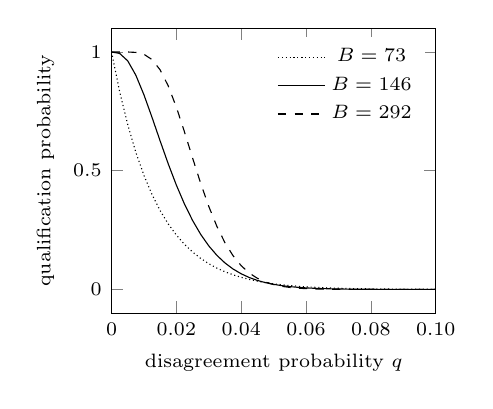
\begin{tikzpicture}[baseline=(current bounding box.north)]
\begin{axis}[width=0.47\linewidth,height=5.2cm,xmin=0,xmax=0.1,
xlabel={disagreement probability $q$},
ylabel={qualification probability},
xtick={0,0.02,0.04,0.06,0.08,0.10},
xticklabels={0,0.02,0.04,0.06,0.08,0.10},
tick label style={font=\scriptsize},label style={font=\scriptsize},
legend style={font=\scriptsize,draw=none},legend pos=north east]
\addplot[densely dotted,black] coordinates {(0.0000,1.000000) (0.0025,0.832994) (0.0050,0.693561) (0.0075,0.577202) (0.0100,0.480141) (0.0125,0.399217) (0.0150,0.331776) (0.0175,0.275598) (0.0200,0.228825) (0.0225,0.189900) (0.0250,0.157520) (0.0275,0.130600) (0.0300,0.108227) (0.0325,0.089644) (0.0350,0.074215) (0.0375,0.061412) (0.0400,0.050793) (0.0425,0.041989) (0.0450,0.034693) (0.0475,0.028651) (0.0500,0.023650) (0.0525,0.019511) (0.0550,0.016089) (0.0575,0.013260) (0.0600,0.010923) (0.0625,0.008993) (0.0650,0.007400) (0.0675,0.006086) (0.0700,0.005003) (0.0725,0.004111) (0.0750,0.003376) (0.0775,0.002770) (0.0800,0.002273) (0.0825,0.001863) (0.0850,0.001527) (0.0875,0.001250) (0.0900,0.001023) (0.0925,0.000837) (0.0950,0.000684) (0.0975,0.000559) (0.1000,0.000457)};
\addlegendentry{$B=73$}
\addplot[solid,black] coordinates {(0.0000,1.000000) (0.0025,0.993915) (0.0050,0.962516) (0.0075,0.902107) (0.0100,0.819495) (0.0125,0.724218) (0.0150,0.625014) (0.0175,0.528543) (0.0200,0.439212) (0.0225,0.359493) (0.0250,0.290379) (0.0275,0.231838) (0.0300,0.183197) (0.0325,0.143432) (0.0350,0.111368) (0.0375,0.085823) (0.0400,0.065684) (0.0425,0.049955) (0.0450,0.037772) (0.0475,0.028407) (0.0500,0.021257) (0.0525,0.015832) (0.0550,0.011739) (0.0575,0.008669) (0.0600,0.006376) (0.0625,0.004673) (0.0650,0.003412) (0.0675,0.002483) (0.0700,0.001801) (0.0725,0.001303) (0.0750,0.000939) (0.0775,0.000675) (0.0800,0.000484) (0.0825,0.000346) (0.0850,0.000247) (0.0875,0.000176) (0.0900,0.000125) (0.0925,0.000088) (0.0950,0.000062) (0.0975,0.000044) (0.1000,0.000031)};
\addlegendentry{$B=146$}
\addplot[dashed,black] coordinates {(0.0000,1.000000) (0.0025,0.999999) (0.0050,0.999867) (0.0075,0.998172) (0.0100,0.990127) (0.0125,0.967970) (0.0150,0.924489) (0.0175,0.856715) (0.0200,0.767278) (0.0225,0.663225) (0.0250,0.553548) (0.0275,0.446780) (0.0300,0.349434) (0.0325,0.265422) (0.0350,0.196236) (0.0375,0.141518) (0.0400,0.099742) (0.0425,0.068828) (0.0450,0.046575) (0.0475,0.030952) (0.0500,0.020226) (0.0525,0.013012) (0.0550,0.008250) (0.0575,0.005159) (0.0600,0.003185) (0.0625,0.001943) (0.0650,0.001172) (0.0675,0.000699) (0.0700,0.000413) (0.0725,0.000241) (0.0750,0.000140) (0.0775,0.000080) (0.0800,0.000046) (0.0825,0.000026) (0.0850,0.000014) (0.0875,0.000008) (0.0900,0.000004) (0.0925,0.000002) (0.0950,0.000001) (0.0975,0.000001) (0.1000,0.000000)};
\addlegendentry{$B=292$}
\end{axis}\end{tikzpicture}%
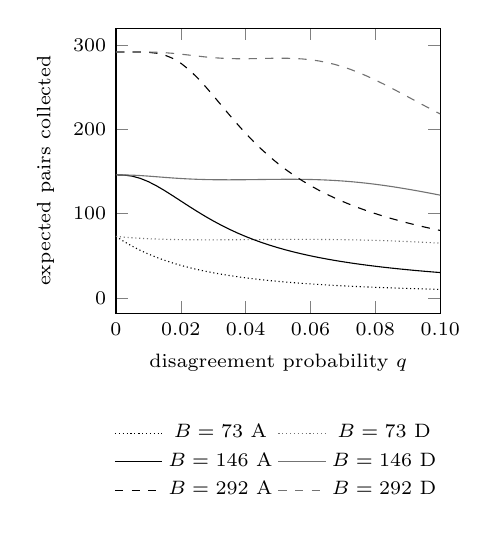
\begin{tikzpicture}[baseline=(current bounding box.north)]
\begin{axis}[width=0.47\linewidth,height=5.2cm,xmin=0,xmax=0.1,
xlabel={disagreement probability $q$},
ylabel={expected pairs collected},
xtick={0,0.02,0.04,0.06,0.08,0.10},
xticklabels={0,0.02,0.04,0.06,0.08,0.10},
tick label style={font=\scriptsize},label style={font=\scriptsize},
legend style={font=\scriptsize,draw=none,at={(0.5,-0.35)},anchor=north,legend columns=2}]
\addplot[densely dotted,black] coordinates {(0.0000,73.000000) (0.0025,66.802289) (0.0050,61.287726) (0.0075,56.373102) (0.0100,51.985854) (0.0125,48.062670) (0.0150,44.548274) (0.0175,41.394373) (0.0200,38.558749) (0.0225,36.004465) (0.0250,33.699182) (0.0275,31.614563) (0.0300,29.725759) (0.0325,28.010955) (0.0350,26.450989) (0.0375,25.029011) (0.0400,23.730186) (0.0425,22.541445) (0.0450,21.451259) (0.0475,20.449447) (0.0500,19.527009) (0.0525,18.675978) (0.0550,17.889296) (0.0575,17.160698) (0.0600,16.484620) (0.0625,15.856112) (0.0650,15.270765) (0.0675,14.724645) (0.0700,14.214239) (0.0725,13.736404) (0.0750,13.288326) (0.0775,12.867478) (0.0800,12.471593) (0.0825,12.098629) (0.0850,11.746745) (0.0875,11.414283) (0.0900,11.099741) (0.0925,10.801761) (0.0950,10.519111) (0.0975,10.250674) (0.1000,9.995432)};
\addlegendentry{$B=73$ A}
\addplot[densely dotted,black!55] coordinates {(0.0000,73.000000) (0.0025,72.055123) (0.0050,71.285161) (0.0075,70.663144) (0.0100,70.166226) (0.0125,69.775058) (0.0150,69.473235) (0.0175,69.246818) (0.0200,69.083921) (0.0225,68.974349) (0.0250,68.909282) (0.0275,68.881005) (0.0300,68.882688) (0.0325,68.908188) (0.0350,68.951907) (0.0375,69.008669) (0.0400,69.073631) (0.0425,69.142225) (0.0450,69.210112) (0.0475,69.273166) (0.0500,69.327468) (0.0525,69.369307) (0.0550,69.395199) (0.0575,69.401901) (0.0600,69.386435) (0.0625,69.346106) (0.0650,69.278524) (0.0675,69.181621) (0.0700,69.053660) (0.0725,68.893247) (0.0750,68.699333) (0.0775,68.471209) (0.0800,68.208502) (0.0825,67.911163) (0.0850,67.579450) (0.0875,67.213910) (0.0900,66.815355) (0.0925,66.384840) (0.0950,65.923635) (0.0975,65.433197) (0.1000,64.915142)};
\addlegendentry{$B=73$ D}
\addplot[solid,black] coordinates {(0.0000,146.000000) (0.0025,145.770094) (0.0050,144.502876) (0.0075,141.866741) (0.0100,137.945151) (0.0125,132.999610) (0.0150,127.339959) (0.0175,121.258739) (0.0200,115.002598) (0.0225,108.764142) (0.0250,102.684297) (0.0275,96.859361) (0.0300,91.349533) (0.0325,86.187209) (0.0350,81.384282) (0.0375,76.938164) (0.0400,72.836549) (0.0425,69.061031) (0.0450,65.589784) (0.0475,62.399466) (0.0500,59.466541) (0.0525,56.768140) (0.0550,54.282607) (0.0575,51.989798) (0.0600,49.871220) (0.0625,47.910054) (0.0650,46.091116) (0.0675,44.400759) (0.0700,42.826765) (0.0725,41.358217) (0.0750,39.985375) (0.0775,38.699552) (0.0800,37.493000) (0.0825,36.358804) (0.0850,35.290787) (0.0875,34.283422) (0.0900,33.331758) (0.0925,32.431351) (0.0950,31.578206) (0.0975,30.768724) (0.1000,29.999653)};
\addlegendentry{$B=146$ A}
\addplot[solid,black!55] coordinates {(0.0000,146.000000) (0.0025,145.950665) (0.0050,145.696614) (0.0075,145.210419) (0.0100,144.551958) (0.0125,143.804283) (0.0150,143.043824) (0.0175,142.329181) (0.0200,141.699294) (0.0225,141.175818) (0.0250,140.766909) (0.0275,140.471007) (0.0300,140.280035) (0.0325,140.181793) (0.0350,140.161629) (0.0375,140.203492) (0.0400,140.290548) (0.0425,140.405524) (0.0450,140.530892) (0.0475,140.649018) (0.0500,140.742329) (0.0525,140.793528) (0.0550,140.785880) (0.0575,140.703545) (0.0600,140.531944) (0.0625,140.258121) (0.0650,139.871082) (0.0675,139.362073) (0.0700,138.724781) (0.0725,137.955449) (0.0750,137.052895) (0.0775,136.018438) (0.0800,134.855744) (0.0825,133.570597) (0.0850,132.170617) (0.0875,130.664944) (0.0900,129.063901) (0.0925,127.378651) (0.0950,125.620869) (0.0975,123.802432) (0.1000,121.935147)};
\addlegendentry{$B=146$ D}
\addplot[dashed,black] coordinates {(0.0000,292.000000) (0.0025,291.999967) (0.0050,291.995209) (0.0075,291.929068) (0.0100,291.587389) (0.0125,290.555227) (0.0150,288.315976) (0.0175,284.425351) (0.0200,278.651092) (0.0225,271.021827) (0.0250,261.791394) (0.0275,251.356482) (0.0300,240.166537) (0.0325,228.651073) (0.0350,217.173982) (0.0375,206.013524) (0.0400,195.361398) (0.0425,185.333269) (0.0450,175.984349) (0.0475,167.325635) (0.0500,159.338357) (0.0525,151.985545) (0.0550,145.220632) (0.0575,138.993391) (0.0600,133.253783) (0.0625,127.954229) (0.0650,123.050811) (0.0675,118.503742) (0.0700,114.277417) (0.0725,110.340204) (0.0750,106.664108) (0.0775,103.224401) (0.0800,99.999233) (0.0825,96.969281) (0.0850,94.117423) (0.0875,91.428451) (0.0900,88.888825) (0.0925,86.486453) (0.0950,84.210509) (0.0975,82.051273) (0.1000,79.999995)};
\addlegendentry{$B=292$ A}
\addplot[dashed,black!55] coordinates {(0.0000,292.000000) (0.0025,291.999990) (0.0050,291.998551) (0.0075,291.979896) (0.0100,291.890822) (0.0125,291.644600) (0.0150,291.161181) (0.0175,290.410730) (0.0200,289.430725) (0.0225,288.312766) (0.0250,287.172847) (0.0275,286.121283) (0.0300,285.242134) (0.0325,284.584465) (0.0350,284.162911) (0.0375,283.963346) (0.0400,283.949930) (0.0425,284.071276) (0.0450,284.264926) (0.0475,284.460402) (0.0500,284.581580) (0.0525,284.549196) (0.0550,284.283969) (0.0575,283.710466) (0.0600,282.761417) (0.0625,281.381977) (0.0650,279.533314) (0.0675,277.195029) (0.0700,274.366086) (0.0725,271.064171) (0.0750,267.323645) (0.0775,263.192411) (0.0800,258.728131) (0.0825,253.994227) (0.0850,249.056062) (0.0875,243.977598) (0.0900,238.818727) (0.0925,233.633352) (0.0950,228.468209) (0.0975,223.362347) (0.1000,218.347161)};
\addlegendentry{$B=292$ D}
\end{axis}\end{tikzpicture}%
\caption{Budget choice under independent pair indicators. Both collection
modes have the same qualification probability (left). Expected collection
length (right) can be lower when only qualification matters (A, black) than
when the three-way result must be preserved (D, grey). These are model
calculations at $\epsilon=0.05$ and 95\% confidence, not observed savings.}
\label{fig:budget-cost}\end{figure}
